%
% Main document
% ===========================================================================
% This is part of the document "Project documentation template".
% Authors: brd3, kaa1
%
%---------------------------------------------------------------------------
\documentclass[
    a4paper,                    % paper format
    10pt,                           % fontsize
    %twoside,                    % double-sided
    openright,              % begin new chapter on right side
    notitlepage,            % use no standard title page
    parskip=half,           % set paragraph skip to half of a line
]{scrreprt}                 % KOMA-script report
%---------------------------------------------------------------------------
\raggedbottom{}
%\KOMAoptions{cleardoublepage=plain}         % Add header and footer on blank pages


% Load Standard Packages:
%---------------------------------------------------------------------------
\usepackage[standard-baselineskips]{cmbright}

\usepackage[ngerman]{babel}                                     % german hyphenation
\usepackage[utf8]{inputenc}
\usepackage[T1]{fontenc}                                            % hyphenation of words with ä,ö and ü
\usepackage{textcomp}                                                   % additional symbols
\usepackage{ae}                                                             % better resolution of Type1-Fonts 
\usepackage{fancyhdr}                                                   % simple manipulation of header and footer 
\usepackage{etoolbox}                                                   % color manipulation of header and footer
\usepackage{graphicx}                           % integration of images
\usepackage{float}                                                      % floating objects
\usepackage{caption}                                                    % for captions of figures and tables
\usepackage{booktabs}                                                   % package for nicer tables
\usepackage{tocvsec2}                                                   % provides means of controlling the sectional numbering
%\usepackage[style=authoryear-ibid,backend=biber]{biblatex}
%\addbibresource{./datenbanken/bibliography.bib}
%---------------------------------------------------------------------------

% Load Math Packages
%---------------------------------------------------------------------------
\usepackage{amsmath}                            % various features to facilitate writing math formulas
\usepackage{amsthm}                             % enhanced version of latex's newtheorem
\usepackage{amsfonts}                           % set of miscellaneous TeX fonts that augment the standard CM
\usepackage{amssymb}                                                    % mathematical special characters
\usepackage{exscale}                                                    % mathematical size corresponds to textsize
%---------------------------------------------------------------------------

% Package to facilitate placement of boxes at absolute positions
%---------------------------------------------------------------------------
\usepackage[absolute]{textpos}
\setlength{\TPHorizModule}{1mm}
\setlength{\TPVertModule}{1mm}
%---------------------------------------------------------------------------                    
            
% Definition of Colors
%---------------------------------------------------------------------------
\RequirePackage{color}                          % Color (not xcolor!)
\definecolor{linkblue}{rgb}{0,0,0.8}            % Standard
\definecolor{darkblue}{rgb}{0,0.08,0.45}        % Dark blue
\definecolor{bfhgrey}{rgb}{0.41,0.49,0.57}      % BFH grey
%\definecolor{linkcolor}{rgb}{0,0,0.8}              % Blue for the web- and cd-version!
\definecolor{linkcolor}{rgb}{0,0,0}                 % Black for the print-version!
%---------------------------------------------------------------------------

% Hyperref Package (Create links in a pdf)
%---------------------------------------------------------------------------
\usepackage[
    pdftex,ngerman,bookmarks,plainpages=false,pdfpagelabels,
    backref = {false},                                      % No index backreference
    colorlinks = {true},                  % Color links in a PDF
    hypertexnames = {true},               % no failures "same page(i)"
    bookmarksopen = {true},               % opens the bar on the left side
    bookmarksopenlevel = {0},             % depth of opened bookmarks
    pdftitle = {Template für Bachelor Thesis},      % PDF-property
    pdfauthor = {brd3},                           % PDF-property
    pdfsubject = {LaTeX Template},        % PDF-property
    linkcolor = {linkcolor},              % Color of Links
    citecolor = {linkcolor},              % Color of Cite-Links
    urlcolor = {linkcolor},               % Color of URLs
]{hyperref}
%---------------------------------------------------------------------------
% Set up page dimension
%---------------------------------------------------------------------------
\usepackage{geometry}
\geometry{a4paper,
    left=28mm,
    right=15mm,
    top=30mm,
    headheight=20mm,
    headsep=10mm,
    textheight=242mm,
    footskip=15mm
}
%---------------------------------------------------------------------------

% Makeindex Package
%---------------------------------------------------------------------------
\usepackage{makeidx}                                % To produce index
\makeindex                                      % Index-Initialisation
%---------------------------------------------------------------------------

% Glossary Package
%---------------------------------------------------------------------------
% the glossaries package uses makeindex
% if you use TeXnicCenter do the following steps:
%  - Goto "Ausgabeprofile definieren" (ctrl + F7)
%  - Select the profile "LaTeX => PDF"
%  - Add in register "Nachbearbeitung" a new "Postprozessoren" point named Glossar
%  - Select makeindex.exe in the field "Anwendung" ( ..\MiKTeX x.x\miktex\bin\makeindex.exe )
%  - Add this [ -s "%tm.ist" -t "%tm.glg" -o "%tm.gls" "%tm.glo" ] in the field "Argumente"
%
% for futher informations go to http://ewus.de/tipp-1029.html
%---------------------------------------------------------------------------
\usepackage[nonumberlist]{glossaries}
\makeglossaries{}

% das zügs do unde dra find i eigendli unnötig, wenn mir so afön fülle mir sitewiss mit "`unüebliche"' begriffe! :(
\newglossaryentry{UML}{name={Wissensmodellierung},description={...}}
\newglossaryentry{Relationale Datenbank}{name={Beschreibungslogik },description={Reasoner ...}}
\newglossaryentry{Relationale Datenspeicherung}{name={Beschreibungslogik },description={Reasoner ...}}
\newglossaryentry{Semantische Datenbank}{name={Beschreibungslogik },description={Reasoner ...}}
\newglossaryentry{Expertensystem}{name={Beschreibungslogik },description={Reasoner ...}}
\newglossaryentry{Ontologie}{name={Ontologie},description={...}}
\newglossaryentry{Domäne}{name={Beschreibungslogik },description={Reasoner ...}}
\newglossaryentry{Wissensdomäne}{name={Beschreibungslogik },description={Reasoner ...}}
\newglossaryentry{Problemdomäne}{name={Beschreibungslogik },description={Reasoner ...}}
\newglossaryentry{Reasoner}{name={Beschreibungslogik },description={Reasoner ...}}
\newglossaryentry{Inferenzmaschine}{name={Beschreibungslogik },description={Reasoner ...}}
\newglossaryentry{Tutorial}{name={Beschreibungslogik },description={Reasoner ...}}
\newglossaryentry{RDF/XML}{name={Resolution},description={...}}
\newglossaryentry{OWL/XML}{name={Parser },description={...}}

\newglossaryentry{Semantik}{name={Inferenz},description={...}}
\newglossaryentry{Knowledge-Engineering}{name={Wissensmodellierung},description={...}}
\newglossaryentry{Knowledge-Engineer}{name={Wissensingeneur},description={Analytiker, Informationsmanager mit entsprechender Methodik und entsprechenden Werkzeugen}}
\newglossaryentry{HERMES}{name={Resolution},description={...}}
\newglossaryentry{Scrum}{name={Inferenz},description={...}}
\newglossaryentry{RDF}{name={Resolution},description={...}}
\newglossaryentry{OWL}{name={Inferenz},description={...}}
\newglossaryentry{Ontologie-Sprache}{name={Inferenz},description={...}}
\newglossaryentry{SWRL}{name={Inferenz},description={...}}
\newglossaryentry{SPARQL}{name={Inferenz},description={...}}
\newglossaryentry{W3C}{name={Inferenz},description={...}}
\newglossaryentry{Apache Stanbol}{name={Inferenz},description={...}}
\newglossaryentry{Stanford Protégé}{name={Inferenz},description={...}}
\newglossaryentry{Clark & Parsia Stardog}{name={Inferenz},description={...}}
\newglossaryentry{XML}{name={Inferenz},description={...}}
\newglossaryentry{Graphdatenbank}{name={Beschreibungslogik },description={Reasoner ...}}
\newglossaryentry{yWorks yEd}{name={Beschreibungslogik },description={Reasoner ...}}
\newglossaryentry{Unifikation}{name={Beschreibungslogik },description={Reasoner ...}}
\newglossaryentry{Semantisches Netz}{name={Parser },description={...}}
\newglossaryentry{NP-vollständig}{name={Parser },description={...}}
\newglossaryentry{URL}{name={Parser },description={...}}
\newglossaryentry{Turtle}{name={Parser },description={...}}
\newglossaryentry{FACT++}{name={Parser },description={...}}
\newglossaryentry{Pellet}{name={Beschreibungslogik },description={Reasoner ...}}
\newglossaryentry{SNARL}{name={Beschreibungslogik },description={Reasoner ...}}
%bis 6.2.1 ok
\newglossaryentry{Resolution}{name={Resolution},description={...}}
\newglossaryentry{Inferenz}{name={Inferenz},description={...}}

\newglossaryentry{Wissensakquise}{name={Wissensakquise},description={Sammeln/ erfassen, aufarbeiten/strukturieren von Wissen}}
\newglossaryentry{Parser}{name={Parser },description={...}}

\newglossaryentry{Beschreibungslogik}{name={Beschreibungslogik },description={Reasoner ...}}
\newglossaryentry{Frame}{name={Parser },description={...}}
\newglossaryentry{Wissensnetzte }{name={Parser },description={...}}

\newglossaryentry{Konzepte}{name={Parser },description={...}}
\newglossaryentry{Axiome}{name={Parser },description={...}}
\newglossaryentry{Prinzipien}{name={Parser },description={...}}
\newglossaryentry{Wissensmodellierung}{name={Beschreibungslogik },description={Reasoner ...}}

\newglossaryentry{Semantisches Web}{name={Beschreibungslogik },description={Reasoner ...}}
\newglossaryentry{Semantik}{name={Beschreibungslogik },description={Reasoner ...}}
\newglossaryentry{Formale Sprache}{name={Beschreibungslogik },description={Reasoner ...}}
\newglossaryentry{Künstliche Intelligenz}{name={Beschreibungslogik },description={Reasoner ...}}
\newglossaryentry{Aussagenlogik}{name={Beschreibungslogik },description={Reasoner ...}}
\newglossaryentry{Prädikatenlogik}{name={Beschreibungslogik },description={Reasoner ...}}

\newglossaryentry{Hierarchische Datenbank}{name={Beschreibungslogik },description={Reasoner ...}}
%\newglossaryentry{Graph}{name={Beschreibungslogik },description={Reasoner ...}}
%\newglossaryentry{Zyklenfreie Nachbarschaft}{name={Beschreibungslogik },description={Reasoner ...}}
%\newglossaryentry{Entität}{name={Beschreibungslogik },description={Reasoner ...}}
%\newglossaryentry{Knoten}{name={Beschreibungslogik },description={Reasoner ...}}
%\newglossaryentry{Kanten}{name={Beschreibungslogik },description={Reasoner ...}}
\newglossaryentry{Existenzaussage}{name={Beschreibungslogik },description={Reasoner ...}}
\newglossaryentry{Ontologiesprache}{name={Beschreibungslogik },description={Reasoner ...}}

\newglossaryentry{Modus Ponens}{name={Beschreibungslogik },description={Reasoner ...}}
\newglossaryentry{Theorem}{name={Beschreibungslogik },description={Reasoner ...}}

\newglossaryentry{Tableau-Kalkül}{name={Beschreibungslogik },description={Reasoner ...}}
\newglossaryentry{Prämisse}{name={Beschreibungslogik },description={Reasoner ...}}
\newglossaryentry{Konklusion}{name={Beschreibungslogik },description={Reasoner ...}}
\newglossaryentry{Literal}{name={Beschreibungslogik },description={Reasoner ...}}
\newglossaryentry{xxx}{name={Beschreibungslogik },description={Reasoner ...}}


%---------------------------------------------------------------------------

% Intro:
%---------------------------------------------------------------------------
%\begin{document}                                % Start Document
\settocdepth{section}                                                       % Set depth of toc
\pagenumbering{roman}                                                       
%---------------------------------------------------------------------------

\providecommand{\titel}{Titel des Berichts}		%  Hier den Titel des Berichts/Thesis eingeben                  % Titel der Arbeit aus Datei titel.tex lesen
\providecommand{\versionnumber}{0.1}			%  Hier die aktuelle Versionsnummer eingeben
\providecommand{\versiondate}{08.06.2014}		%  Hier das Datum der aktuellen Version eingeben
                % Versionsnummer und -datum aus Datei version.tex lesen

% Set up header and footer
%---------------------------------------------------------------------------
\makeatletter
\patchcmd{\fancyhead}{\rlap}{\color{bfhgrey}\rlap}{}{}     % new color of header
\patchcmd{\fancyfoot}{\rlap}{\color{bfhgrey}\rlap}{}{}     % new color of footer
\makeatother

\fancyhf{}                                                                      % clean all fields
\fancypagestyle{plain}{% new definition of plain style 
    \fancyfoot[OR,EL]{\footnotesize \thepage}   % footer right part --> page number
    \fancyfoot[OL,ER]{\footnotesize \titel, Version \versionnumber, \versiondate}   % footer even page left part 
}

\renewcommand{\chaptermark}[1]{\markboth{\thechapter.  #1}{}}
\renewcommand{\headrulewidth}{0pt}              % no header stripline
\renewcommand{\footrulewidth}{0pt}              % no bottom stripline

\pagestyle{plain}
%---------------------------------------------------------------------------

\begin{document}

% Title Page and Abstract
%---------------------------------------------------------------------------
%%
% Project documentation template
% ===========================================================================
% This is part of the document "Project documentation template".
% Authors: brd3, kaa1
%

\begin{titlepage}


% BFH-Logo absolute placed at (28,12) on A4 
% Actually not a realy satisfactory solution but working.
%---------------------------------------------------------------------------
\setlength{\unitlength}{1mm}
\begin{textblock}{20}[0,0](28,12)
	
\includegraphics[scale=1.0]{bilder/BFH_Logo_B.png}
\end{textblock}
\color{black}

% Institution / Titel / Untertitel / Autoren / Experten:
%---------------------------------------------------------------------------
\begin{flushleft}

\vspace*{21mm}

\fontsize{26pt}{40pt}\selectfont 
\titel 				\\							% Titel aus der Datei vorspann/titel.tex lesen
\vspace{2mm}

\fontsize{16pt}{24pt}\selectfont\vspace{0.3em}
Hier steht ein Untertitel 			\\							% Untertitel eingeben
\vspace{5mm}

\fontsize{10pt}{12pt}\selectfont
\textbf{Art der Arbeit (Semesterarbeit / Bachelorthesis / etc.)} \\									% eingeben
\vspace{7mm}

% Abstract (eingeben):
%---------------------------------------------------------------------------
\begin{textblock}{150}(28,100)
\fontsize{10pt}{12pt}\selectfont
[Kurztext (Abstract) einf�gen, falls gew�nscht] \\ 
Dieses Dokument dient als Vorlage f�r die Erstellung von Berichten nach den Richtlinien der BFH. Die Vorlage ist in \LaTeX{} erstellt und unterst�tzt das automatische Erstellen von diversen Verzeichnissen, Literaturangaben, Indexierung und Glossaren. Dieser kleine Text ist eine Zusammenfassung �ber das vorliegenden Dokument mit einer L�nge von 4 bis max. 8 Zeilen. \\
Das Titelbild kann in den Zeilen 157/158 der Datei template.tex ein- oder ausgeschaltet werden.
\end{textblock}

\begin{textblock}{150}(28,225)
\fontsize{10pt}{17pt}\selectfont
\begin{tabbing}
xxxxxxxxxxxxxxx\=xxxxxxxxxxxxxxxxxxxxxxxxxxxxxxxxxxxxxxxxxxxxxxx \kill
Studiengang:	\> [z.B. Elektro- und Kommunikationstechnik]	\\			% Namen eingeben
Autoren:		\> [Test Peter, M�ster R�s�]		\\					% Namen eingeben
Betreuer:	\> [Dr.~Xxxx Xxxx, Dr.~Yyyy Yyyy]		\\					% Namen eingeben
Auftraggeber:	\> [Wwwww AG]						\\					% Namen eingeben
Experten:		\> [Dr.~Zzzz Zzzz]				\\					% Namen eingeben
Datum:			\> \versiondate					\\		% aus Datei vorspann/version.tex lesen
\end{tabbing}

\end{textblock}
\end{flushleft}

\begin{textblock}{150}(28,280)
\noindent 
\color{bfhgrey}\fontsize{9pt}{10pt}\selectfont
Berner Fachhochschule | Haute �cole sp�cialis�e bernoise | Bern University of Applied Sciences
\color{black}\selectfont
\end{textblock}


\end{titlepage}

%
% ===========================================================================
% EOF
%
        % activate for Titelseite ohne Bild
%
% Project documentation template
% ===========================================================================
% This is part of the document "Project documentation template".
% Authors: brd3, kaa1
%

\begin{titlepage}


% BFH-Logo absolute placed at (28,12) on A4 and picture (16:9 or 15cm x 8.5cm)
% Actually not a realy satisfactory solution but working.
%---------------------------------------------------------------------------
\setlength{\unitlength}{1mm}
\begin{textblock}{20}[0,0](28,12)
    
\includegraphics[scale=1.0]{bilder/BFH_Logo_B.png}
\end{textblock}

\begin{textblock}{154}(28,48)
    \begin{picture}(150,2)
        \put(0,0){\color{bfhgrey}\rule{150mm}{2mm}}
    \end{picture}
\end{textblock}

\begin{textblock}{154}[0,-0.2](28,42)
    \centering
    
\includegraphics[scale=0.7]{bilder/owl.png}   % Titelbild definieren
\end{textblock}

\begin{textblock}{154} (28,135)
    \begin{picture}(150,2)
        \put(0,0){\color{bfhgrey}\rule{150mm}{2mm}}
    \end{picture}
\end{textblock}
\color{black}

% Institution / Titel / Untertitel / Autoren / Experten:
%---------------------------------------------------------------------------
\begin{flushleft}

\vspace*{120mm}

\fontsize{26pt}{28pt}\selectfont
\titel% Titel aus der Datei vorspann/titel.tex lesen
\vspace{3mm}



\fontsize{10pt}{12pt}\selectfont
\textbf{Aufbau von Wissensdomänen anhand einer semantischen Datenbank} \\                                 % eingeben
\vspace{3mm}

\begin{textblock}{150} (28,215)
\fontsize{10pt}{17pt}\selectfont
\begin{tabbing}
xxxxxxxxxxxxxxx\=xxxxxxxxxxxxxxxxxxxxxxxxxxxxxxxxxxxxxxxxxxxxxxx \kill
Autoren:        \> Sven Osterwalder, Mira Günzburger     \\                  % Namen eingeben
Datum:          \> \versiondate\\      % aus Datei vorspann/version.tex lesen
\end{tabbing}

\end{textblock}
\end{flushleft}

\begin{textblock}{150} (28,280)
\noindent 
\color{bfhgrey}\fontsize{9pt}{10pt}\selectfont
Berner Fachhochschule | Haute école spécialisée bernoise | Bern University of Applied Sciences
\color{black}\selectfont
\end{textblock}


\end{titlepage}

%
% ===========================================================================
% EOF
%
          % activate for Titelseite mit Bild
\cleardoublepage{}
\phantomsection{}
% Versionenkontrolle :
% -----------------------------------------------

\begin{textblock}{180} (15,150)
\color{black}
\begin{huge}
Versionen
\end{huge}
\vspace{10mm}

\fontsize{10pt}{18pt}\selectfont
\begin{tabbing}
xxxxxxxxxxx\=xxxxxxxxxxxxxxx\=xxxxxxxxxxxxxx\=xxxxxxxxxxxxxxxxxxxxxxxxxxxxxxxxxxxxxxxxxxxxxxx \kill
Version	\> Datum	\> Status		\> Bemerkungen		\\
0.1	\> 08.06.2014	\> Entwurf		\> Anforderungsdokument erstellen	\\	
0.2	\> 08.08.2014	\> Entwurf		\> Korrekturen und Ergänzungen	\\	
0.3	\> 19.09.2014	\> Entwurf		\> Anpassungen an die Aufgabenstellung	\\ 
%0.3	\> 02.09.2013	\> Entwurf		\> Donec eget aliquam urna. Lorem ipsum dolor sit amet	\\ 
%1.0	\> 12.09.2013	\> Definitiv	\> Lorem ipsum dolor sit ametPhasellus scelerisque, leo sed iaculis ornare 	\\ 
%1.1	\> 04.11.2013	\> Korrektur	\> Layout angepasst	\\
\end{tabbing}

\end{textblock}

\phantomsection{}
\cleardoubleemptypage{}
\setcounter{page}{1}
\cleardoublepage{}
\phantomsection{}
\addcontentsline{toc}{chapter}{Versionen}
\cleardoubleemptypage{}
%---------------------------------------------------------------------------

% Table of contents
%---------------------------------------------------------------------------
\tableofcontents
\cleardoublepage{}
%---------------------------------------------------------------------------

% Main part:
%---------------------------------------------------------------------------
\pagenumbering{arabic}
\chapter{Einleitung}
\label{chap:einleitung}

%CHeckliste fausibibel
%Ausgangslage, Problemstellung
%• Auftrag oder Aufgabenstellung
%• Resultat der Arbeit
%• Methodik (Herkunft der Daten, Vorgehen, Systemund
%Gültigkeitsgrenzen)
%• Folgerungen, offene Fragen

Der klassische Ansatz der Wissensabbildung, zum Beispiel in Form von UML, welchem die relationale Datenspeicherung zugrunde liegt, wird in der heutigen Informatik weitläufig eingesetzt und ist de facto Standard. Häufig geschieht dies in enger Verbindung mit der objektorientierten Programmierung. Experten aus einer Fachrichtung sind fähig diese Daten zu interpretieren und daraus Schlüsse zu ziehen. Es ist aber nicht möglich automatisch Fragestellungen zu beantworten, welche über reine Relationsverknüpfungen hinausgehen. Mit dieser Technik sind Objekteigenschaften und -Verhalten also eher schwer abbildbar. Eine andere Art Wissen zu repräsentieren sind semantische Datenbanken. Diese ermöglichen das Abbilden des Objektverhaltens und können mithilfe von Schlussfolgerungen die Rolle des Experten einnehmen.

In dieser Bachelorthesis soll eine solche semantische Datenbank aufgebaut und angewendet werden.  Die Arbeit wurde in zwei Teilen umgesetzt: Einem  theoretischen und einem praktischen Teil. Der theoretische Teil zeigt in Form eines Tutorials auf, wie ein knowledge engineer bei der Wissensmodellierung vorgeht. Er nutzt dabei Ontologien als Basis, um eine semantische Datenbank aufzubauen. Im praktischen Teil soll eine solche Ontologie aufgebaut und per Benutzerschnittstelle zugänglich gemacht werden.

Die gesteckten Ziele konnten allesamt erreicht werden. Es ist den Autoren gelungen die Theorie der Wissensmodellierung übersichtlich in einem Dokument aufzubereiten und wiederzugeben. Speziell dabei ist, dass in diesem fachliche Grundlagen mit einem praktischen Beispiel verbunden werden. Zusätzlich konnten auch konkrete Tipps aus der eigenen Erfahrung eingeflochten werden. Dieses Dokument ist dem Abschlussdokument als Anhang beigefügt.

Im praktischen Teil der Arbeit wurde ein Expertensystem für Reisen aufgebaut: ``In der heutigen Zeit werden Ferien häufig per Internet gebucht. Was aber, wenn der Urlaub nicht einfach zwei Wochen an einem Ort stattfinden soll? Was, wenn der Kunde reisen möchte? Oder sonstige spezielle Wünsche hat? Für solche Anforderungen muss er auch heute noch in ein Reisebüro um sich beraten zu lassen.''\\
Bei der Automatisierung dieses Prozesses kommt die Ontologie ins Spiel, welche mithilfe von Eigenschaften, Kriterien und Regeln die Problemdomäne abbildet. Durch die Verwendung eines Reasoners können verschiedene Reisevorschläge gemacht werden.\\
Um eine sehr individuelle Reiseplanung zu erreichen, musste zuerst eine Ontologie in Form von Klassen, Individuen, Relationen und Eigenschaften erstellt werden. Ohne klaren Rahmen würde eine Ontologie zu komplex und zu gross. Daher bauten die Autoren die Ontologie anhand exemplarischer Tages und Wochenendausflügen in der Schweiz auf.\\
Als Ergebnis können die Autoren eine semantischen Datenbank präsentieren. Dabei wird die von ihnen gewählte Problemdomäne in einem klar gesteckten Rahmen abgedeckt und die Mächtigkeit der Wissensmodellierung veranschaulicht. Die Schnittstelle für Benutzer wurde in Form eines Assistenten umgesetzt, welcher den Benutzer durch die Möglichkeiten führt und ihn bei der Planung seiner Reise unterstützt. Damit konnten die Autoren verhindern, dass Benutzer gezwungen sind, Abfragen in einer komplexen Abfragesprache zu formulieren.

Die Wissensmodellierung auf Basis von Ontolgien ist auf ihre Weise eine mächtiges Werkzeug um Informationen mit Semantik zu versehen. Trotzdem hat diese Art der Modellierung gewisse Einschränkungen, welche von anderen auf Logik basierenden Sprachen, wie zum Beispiel Prolog, abgedeckt werden. Im Laufe der Arbeit erkannten die Autoren, dass es noch Bedarf an Weiterentwicklung im Bezug auf die angebotenen Werkzeuge gibt. So musste eine Kombination von zwei Werkzeugen verwendet werden um sämtliche Anforderungen umzusetzen.

% Hier beschreiben Sie kurz das Thema der Arbeit, den Kontext sowie in knappen Worten das Ergebnis. Dieser Abschnitt gleicht einem Management Summary. Ziel dieses Kapitels ist, dem Leser die Entscheidungsgrundlage zu liefern, ob er die Arbeit lesen soll oder nicht.

% Einträge im Verzeichnis erscheinen lassen ohne hier eine Referenz einzufügen
%\nocite{kopka:band1}

\chapter{Wissensdomäne}
\label{chap:wissensdomäne}
Wie sich in der Vorarbeit herausgestellt hat, ist es notwendig die Domäne, in welcher Anfragen gestellt werden sollen, sehr detailliert abzubilden. Zudem ist die technische Umsetzung der Suche mittels Apache Stanbol weniger weit ausgearbeitet als ursprünglich angenommen. Um die Komplexität in einem angemessenen Rahmen zu halten, gilt es die Entitäten, also die Modellierung der Umwelt, stark einzuschränken.
Als Folge dieser Erkenntnisse wird die Wissendomäne, mit welcher gearbeitet wird, eingeschränkt. Bei der gewählten Domäne handelt es sich um die Grundlagen der Programmierung am Beispiel der Programmiersprache Java. Dies erlaubt es, dass der Aufbau der Wissensdatenbank überschaubar bleibt, hat aber den Nachteil, dass nur eine beschränkte Anzahl von Fragestellungen beantwortet werden können.

\chapter{Komponenten}
\label{chap:komponenten}
Ein Expertensystem besteht aus drei Komponenten, wie im~\hyperref[sec:anhang:tutorial_dokument]{Tutorial} unter Kapitel 2 beschrieben.\\
Die Komponenten sind:
\begin{itemize}
    \item Wissensdatenbank: Enthält die Fakten des Problembereiches in formaler Sprache
    \item Inferenz-Maschine: Verarbeitungsmechanismus zum automatischen Ziehen von Schlüssen
    \item Benutzerschnittstelle
\end{itemize}
Wie in~\autoref{ssubsec:vorgehen:grundlagen:technisch} erwähnt, ist die Verwendung von Werkzeugen zur Modellierung einer Ontologie sinnvoll.\\
Dabei gibt es Überschneidungen: \textbf{Komponenten können auch Werkzeuge sein.}

Das folgende Kapitel beschreibt die während dieser Arbeit verwendeten Komponenten und Werkzeuge.

Die Wissensmodellierung sollte ursprünglich mit Hilfe von Apache Stanbol umgesetzt werden, wie unter~\autoref{ssubsec:vorgehen:grundlagen:technisch} erwähnt. Während der Arbeit wurde erkannt, dass diese Technologie für die vorgesehene Aufgabe nur bedingt sinnvoll ist. In Apache Stanbol ist es zwar möglich die modellierte Wissensdomäne zu importieren. Das importierte Modell wird als Ontologie in Form von Tripeln gespeichert. Die Objekte, ihre Eigenschaften sowie Relationen lassen sich jedoch nicht verwalten.

Für Anfragen an die Wissensdatenbank ist eine entsprechende Schnittstelle notwendig. Von Apache Stanbol wird diese Schnittstelle in Form eines SPARQL-Endpoints zur Verfügung gestellt. Der SPARQL-Endpoint nutzt jedoch die ContentHub-Komponente von Apache Stanbol als Datenbasis. Diese stellt nur Wissen zur Verfügung, welches aus angereicherten Inhalten abgeleitet ist. Mittels Ontologien und Regeln werden diese Inhalte angereichert.

Eine aufwändige Recherche ergab: Anderen Datenquellen können für den SPARQL-Endpoint genutzt werden. Dies bedeutet jedoch einen erheblichen Mehraufwand in Form einer eigenen Implementation.

Damit war Apache Stanbol nicht das geeignete Werkzeug für diese Arbeit. Bei weiteren Recherchen wurden weitere Werkzeuge gefunden, welche als Ersatz für Apache Stanbol genutzt werden konnten: \textit{Protégé} der Universität Stanford sowie \textit{Stardog} der Firma Clark \& Parsia.

\section{Stanford Protégé}
\label{sec:komponenten_protege}
Protégé ist eine Entwicklungsumgebung für Ontologien und wurde von den Autoren als \textit{Werkzeug} verwendet. Entwickelt von der Universität Stanford findet es in der Fachwelt häufig Anwendung.\\
Es unterstützt sowohl die Modellierung von Ontologien, wie auch mittels verschiedener Reasoner das Reasoning.

\subsection{Merkmale}
\label{subsec:komponenten_protege_features}
In Protégé können Ontologien in unterschiedlichen Schreibweisen, wie zum Beispiel OWL/XML, Turtle oder RDF/XML eingelesen und abgespeichert werden. Die Dateien tragen immer die Endung ``.owl''. Protégé hält eingelesene Ontologien als Graphstruktur im Speicher~\footnote{\url{http://protegewiki.stanford.edu/wiki/Protege4Features}} und ermöglicht Reasonern den direkten Zugriff auf die Graphstruktur~\footnote{\url{http://protege.stanford.edu/products.php}}.\\
Die Entwicklungsumgebung zeigt verschiedene Ansichten für dieselbe Ontologie. \\
Ausser Anlegen und Bearbeiten einer Ontologie können in Protégé (ab Version 5.0.0 Beta-16) SWRL-Regeln verwaltet werden. Diese werden von Protégé direkt in der Ontologie abgelegt.

Durch das SPARQL-Modul bietet Protégé die Möglichkeit Informationen der Ontologie mittels Abfragen zu gewinnen. Ist zusätzlich ein Reasoner-Modul geladen und aktiviert, kann die Umgebung bei Abfragen Inferenzen einbeziehen. Es können verschiedene Reasoner, wie beispielsweise FACT++ oder Pellet genutzt werden (siehe~\ref{subsec:komponenten_reasoner}).

(vgl.~\cite{protegeFeatures})

\subsection{Ansichten}
\label{subsec:komponenten_protege_view}

Die Benutzerfreundlichkeit von Protégé wird unter Anderem dadurch erreicht, dass verschiedene Sichten auf eine Ontologie geboten werden. Neben der Entitätsansicht (Entity-View, diese enthält sämtliche Elemente einer Ontologie) existiert für alle Elementtypen wie Klassen, Dateneigenschaften, Objekteigenschaften und Individuen eine eigene Ansicht.

Alle Ansichten sind als Baumstruktur organisiert. Dadurch entsteht eine klare Übersicht. Diese wiederum ermöglicht eine Hierarchie-getreue Abbildung des zu Grunde liegenden XML-Dokumentes.

Protégé bietet weitere Ansichten. Beispielsweise kann der Graph einer Ontologie in der OntoGraf-Ansicht betrachtet werden.

\begin{figure}[H]%[htbp]
    \centering
    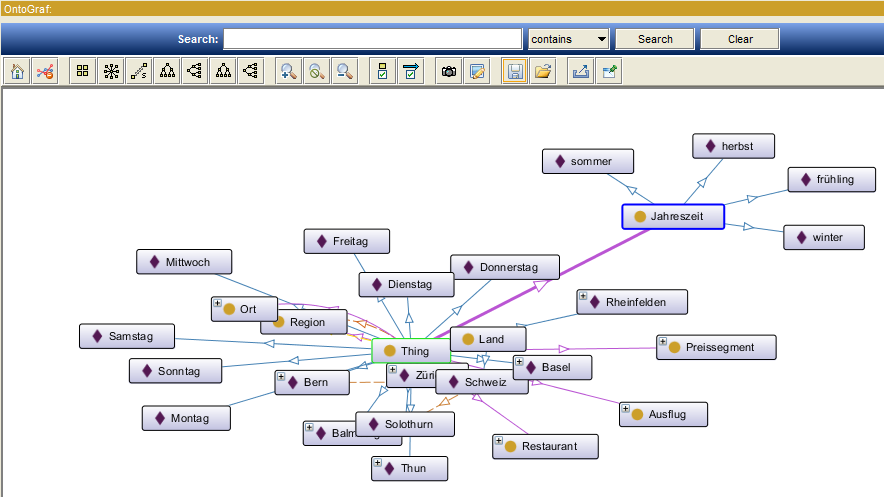
\includegraphics[scale=0.7]{bilder/OntoGraf.png}
    \caption{Beispiel der OntoGraf-Ansicht.\label{fig:kompo:ontograf}\protect\footnotemark}
\end{figure}
\footnotetext{Eigene Darstellung mittels Protégé.}

Schlussfolgerungen werden in allen Ansichten direkt zur Laufzeit des Reasoners bei allen Elementtypen ergänzt.

(vgl.~\cite{protegeView})

\section{Clark \& Parsia Stardog}
\label{sec:komponenten_stardog}
Bei Stardog handelt es sich um eine Graphdatenbank mit Unterstüztung des RDF-Graphenmodelles. Sie bietet den Import und Export von Ontologien in diversen Format an und die Möglichkeit Informationen einer Ontologie mittels SPARQL abzufragen. Des Weiteren unterstützt Stardog die Sprache OWL sowie SWRL-Regeln.\\
Pellet, in Stardog enthalten, bildet eine zentrale Komponente für die Schlussfolgerung.

Stardog bietet viele Kommunikationsschnittstellen, so z.B. HTTP und SNARL.\\
Programmierschnittstellen sind für zahlreiche Sprachen, so beispielsweise Java, JavaScript oder Python vorhanden.

Stardog unterscheidet drei Versionen der Lizenzierung: Community, Developer und Enterprise. Die Versionen unterscheiden sich durch maximale Anzahl der verwaltbaren Datenbanken und der möglichen Tripel pro Datenbank, Anzahl gleichzeitiger Verbindungen und durch Anzahl Benutzer und Rollen. Je nach gewählter Lizenzierung leistet der Hersteller eine Kundenbetreuung.

(vgl.~\cite{stardogDocu})

\subsection{Reasoner}
\label{subsec:komponenten_reasoner}
Reasoner sind Komponenten,  die Folgerungen von implizitem Wissen zulassen bzw.\ anbieten. Es handelt es sich um eine Art ``Verstehen'' der Maschinen. Ziel ist es, aus explizitem Wissen in Form einer Ontologie implizites Wissen zu gewinnen.

Wie bereits unter~\autoref{ssubsec:vorgehen:grundlagen:technisch} erwähnt, wurde Pellet als Reasoner (Anwendung zum Ziehen von Schlüssen) gewählt. Eine detaillierte Beschreibung von Pellet findet sich im~\hyperref[sec:anhang:tutorial_dokument]{Tutorial} unter Abschnitt 6.4.

\subsection{Konkrete Anwendung der Komponenten zur Modellierung der Ontologie}
\label{subsec:komponenten_anwendung}
Im Laufe der Arbeit hat sich herausgestellt, dass das Schlussfolgern in Protégé nicht einwandfrei funktioniert. Gewisse SPARQL-Anfragen wurden nicht erwartungsgemäss beantwortet.

Da sowohl Protégé als auch Stardog dieselbe Komponente für Schlussfolgerungen (den Pellet-Reasoner) verwenden, muss es sich bei dem Fehlverhalten um einen Fehler bei der Aufbereitung der Abfragen handeln.

In Protégé existiert zudem keine HTTP-Schnittstelle. Es existiert zwar eine Programmierschnittstelle mit welcher eine HTTP-Schnittstelle geschaffen werden kann. Dies wurde aus zeitlichen Gründen verworfen.

Angesichts der Funktionsstörung und mangelnder HTTP-Schnittstelle, wurde die Ontologie in Protégé erstellt und bearbeitet. Die Weiterverarbeitung der Ontolgie erfolgte mittels Stardog, da Stardog die SPARQL-Anfragen korrekt beantwortet und ausserdem eine HTTP- und REST-Schnittstelle bietet.

Dafür musste in Stardog eine neue Datenbank erstellt werden. In diese wurde die mittels Protégé vorbereitete Ontologie im RDF/XML-Format eingespielt.

Stardog bietet bei der Verwendung des Reasoners mehr Möglichkeiten als die anderen Werkzeuge (wie zum Beispiel Protégé). Schlussfolgerungen mittels einer Kombination von RDFS-, QL-, RL- und EL-Axiomen sowie zusätzlich SWRL-Regeln gezogen werden. Details finden sich unter~\footnote{\url{http://docs.stardog.com/\#_reasoning_levels}}.


Durch die Kombination dieser beiden Werkzeuge Protégé und Stardog konnte eine zuverlässige Modellierung und Verwendung der Ontologie erreicht werden.

\section{Benuzteroberfläche}
\label{sec:komponenten:ember}
Ein Teil der Aufgabe bestand darin, eine möglichst benutzerfreundliche Schnittstelle zwischen Mensch und System zu entwickeln.\\
Als Schnittstelle haben die Autoren eine Webapplikation zur Reiseplanung entwickelt, wie im~\autoref{sec:loesung_gui} ausgeführt. Diese ermöglicht das Planen einer Reise mit Hilfe eines Assistenten. Der Benutzer kann die gewünschten Reisekriterien auswählen und erhält schliesslich eine Auswahl an Reiseobjekten, welche seinen Kriterien entsprechen.

\subsection{Komponenten der Benutzeroberfläche}
\label{subsec:komponenten:gui:komponenten}
Folgende Komponenten wurden zur Umsetzung der Benutzeroberfläche gewählt:
\begin{itemize}
    \item \textit{Vagrant}\footnote{\url{http://www.vagrantup.com}}\\
        Virtualisierungslösung
    \item \textit{nginx}\footnote{\url{https://nginx.org}}\\
        Webserver
    \item \textit{Ember.js}\footnote{\url{http://emberjs.com}}\\
        Applikations-Framework
    \item \textit{Bootstrap}\footnote{\url{http://getbootstrap.com}}\\
        HTML-, CSS- und JavaScript-Framwork von Twitter
\end{itemize}
(Die Auswahl erfolgte aufgrund beruflicher Erfahrungen der Autoren.)

\subsubsection{Vagrant}
\label{ssubsec:komponenten:gui:komponenten:vagrant}
Bei Vagrant handelt es sich um ein Werkzeug zur Erstellung von vollständigen Entwicklungsumgebungen basierend auf Virtualisierung (vgl.~\cite{vagrant}). Details dazu finden sich unter~\footnote{http://www.vagrantup.com/about.html}.

In der vorliegend Arbeit wurde Vagrant zur Bereitstellung einer (virtuellen) Entwicklungsumgebung genutzt. Dabei wird die eigentliche Anwendung von der Entwicklungsumgebung getrennt. Dadurch kann die Entwicklungsumgebung jederzeit mittels weniger Befehle wieder neu aufgebaut werden.

\subsubsection{nginx}
\label{ssubsec:komponenten:gui:komponenten:nginx}
nginx (``engine x'' ausgesprochen) ist ein freier open-source Webserver. Seine Stärken liegen unter anderem  auf hoher Leistung, hoher Nebenläufigkeit und geringem Speicherverbrauch. Er ist der am zweithäufigsten eingesetzte Webserver (vgl.~\cite{nginx}).

nginx wurde innerhalb der (virtuellen) Entwicklungsumgebung zur Bereitstellung der Applikation genutzt. So kann die Applikation innerhalb eines Rechners wie eine externe Webseite angesprochen werden.

\subsubsection{Ember.js}
\label{ssubsec:komponenten:gui:komponenten:emberjs}
Ember.js ist ein clientseitiges open-source Framework zur Erstellung von Webapplikationen. Es baut auf dem Model-View-Controller (MVC) Softwarearchitektur-Muster auf. Es erlaubt die Erstellung von skalierbaren Anwendungen mittels einer einzigen Datei und bietet dabei deklarative Datenbindung, dynamische Eigenschaften, automatisch aktualisierte Templates sowie eine Zustandsverwaltung der Applikation mittels einer Router-Komponente (vgl.~\cite{ember}).

Ember.js wurde für die Umsetzung der Applikationslogik der Benutzeroberfläche eingesetzt.

\subsubsection{Bootstrap}
\label{ssubsec:komponenten:gui:komponenten:bootstrap}
Bootstrap der Firma Twitter ist eine Sammlung von Werkzeugen um Webseiten und Webapplikationen zu erstellen. Bootstrap bietet unter anderem verschiedene, auf HTML und CSS basierende Vorlagen für Typographie, Formulare, Schaltflächen und Navigation (vgl.~\cite{bootstrap}).

Bootstrap wurde zur grafischen Gestaltung der Benutzeroberfläche eingesetzt.

\subsection{Architektur}
\label{subsec:komponenten:gui:architektur}
\begin{figure}[H]
    \centering \rotatebox{0}{\scalebox{0.5}[0.5]{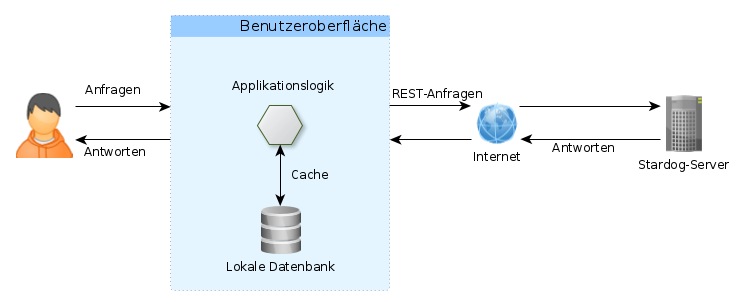
\includegraphics{bilder/architektur_gui.png}}}
    \caption{Architektur der Benutzeroberfläche\label{fig:architektur:gui}\protect\footnotemark}
\end{figure}
\footnotetext{Eigene Darstellung mittels yEd.}

Die obenstehende Abbildung~\ref{fig:architektur:gui} zeigt die Architektur der Benutzeroberfläche, bestehend aus einem Frontend und einem Backend. Mit Frontend ist die Applikation selbst (Benutzeroberfläche) gemeint, mit Backend der Stardog-Server.

Die Applikation besteht aus \textit{Modellen}, \textit{Ansichten} und \textit{Routen}.

\textit{Modelle} sind \textit{Reisen}, \textit{Dateneigenschaften} und \textit{Objektrelationen}.\\
\hangindent=1.5cm Das \textit{Modell} \textit{Reise} entspricht \textit{Individuen}, das \textit{Modell} \textit{Dateneigenschaft} \textit{DataProperties} und\\
das \textit{Modell} \textit{Objektrelation} den \textit{ObjectProperties} der Ontologie.

\textit{Routen} definieren, entsprechend ihrem Namen, den Ablauf der Applikation.\\
\hangindent=1.5cm \textit{Welcome}-Route ist der Einstieg der Applikation. Von der \textit{Welcome}-Route aus werden die \textit{Routen} \textit{Step1}, \textit{Step2} und \textit{Step3} nacheinander in Form eines Schritt-für-Schritt-Assistenten durchlaufen.\\
In Schritt 1 wird die Art der Ausflüge gewählt.\\
In Schritt 2 werden die \textit{Dateneigenschaften} sowie die \textit{Objektrelationen} pro zuvor gewählter Art der Ausflüge gewählt.\\
Schritt 3 gibt alle Instanzen zurück, welche den gewählten Kriterien entsprechen.\\
\\
Da in Schritt 1 nur bestimmte Individuen der Ontologie angezeigt werden sollen, wurden in der Ontologie diese Individuen mit der \textit{Dateneigenschaft} ``reise'' gekennzeichnet. Dadurch beschränkt sich die Abfrage von Schritt 1 nur auf diese Individuen.

Die \textit{Ansichten} kombinieren die Gestaltung (das Layout) der Seite mit der Ansicht der aktuellen Route.

Die gewählte Graphdatenbank Stardog bietet externen Zugriff via REST-Protokoll. Das gewählte Framework Ember.js bietet REST-Unterstützung via REST-Adapter an. Der REST-Adapter implementiert standardmässig Lesen und Schreiben einer REST-Schnittstelle.

Da das Ziel der Arbeit nicht eine vollständige Umsetzung (Lesen und Schreiben) der Ontologie war, wurde der Zugriff auf die Datenbank nur lesend implementiert. Dadurch kann die umgesetzte Applikation und somit der Benutzer Daten der Ontologie nur lesen (und nicht ändern). Daher musste das Standardverhalten des REST-Adapters von Ember.js durch Nutzung der lokalen Datenbank von Ember.js umgangen werden.

Beim initialen Aufruf der Applikation wird die gesamte Ontologie via REST-Protokoll vom Server abgerufen und nur in der lokalen Datenbank von Ember.js in Form der \textit{Modelle} abgelegt. Damit der Benutzer beim initialen Aufruf der Applikation nicht auf den Datenaustausch warten muss und die Applikation nicht blockiert wird, findet der Datenaustausch asynchron statt. Trotz im  Hintergrund laufender Anfragen kann die Applikation benützt werden. Dabei werden die \textit{Modelle} an die \textit{Ansicht} gebunden. Das heisst, erhält die Applikation Daten eines Modells, wird automatisch dessen \textit{Ansicht} dargestellt bzw.\ aktualisiert.

\chapter{Technische Umsetzung}
\label{chap:technischeUmsetzung}
Zur technischen Umsetzung wird, wie in der Abschlussarbeit des Moduls 7302 "`Projekt 2"' evaluiert, Apache Stanbol eingesetzt.
Freundlicherweise steht von der BFH Infrastrukur zum Betrieb zur Verfügung. Der Server steht unter elephantsearch.bfh.ch zur Verfügung.
\chapter{Ziel der Thesis}
\label{chap:thesisziel}
Als Endresultat der Thesis soll ein Dokument mit Tutorial Charakter stehen, welches aufzeigt wie Knowledge Engineers vorgehen, um eine Problemdomäne systematisch zu modellieren und zu formalisieren. 

Es soll also gezeigt werden, wie eine Speicherung von Daten, die Verknüpfung dieser sowie ihre logische Ableitungen in einer Semantischen Datenbank für eine RDF/OWL-Ontologie  umgesetzt wird.~\cite{Aufgabenstellung}

 
Dies wird mittels eines konkreten Anwendungsproblems, der Erlernung der Programmiersprache Prolog, umgesetzt.

\section{Milestones}
\label{sec:Milestones}
Mit der folgenden Auflistung erhält man eine Übersicht, der in dieser Anfangsphase bereits erkennbaren Meilensteine der Thesis:
\begin{itemize}
	\item Anforderungsdokument \\
	\item Analysieren der Modellierung der Entitäten & Attributen \\
	\item Analysieren des Erzeugen der Regeln \\
	\item Analysieren der Sprache SPARQL	\\
	\item Ausformulieren der gewonnenen Erkenntnissen \\
	\item Installieren der nötigen Infrastruktur auf dem BFH Server\\
	\item Einarbeitung der Erzeugten Elemente in Stanbol \\
	\item Erzeugen einer simplen Anwenderoberfläche \\
\end{itemize}


%---------------------------------------------------------------------------

% Glossary
%---------------------------------------------------------------------------
\cleardoublepage{}
\phantomsection{}
\addcontentsline{toc}{chapter}{Glossar}
\renewcommand{\glossaryname}{Glossar}
\printglossary{}
%---------------------------------------------------------------------------

% Bibliography
%---------------------------------------------------------------------------
%\cleardoublepage
\phantomsection{}
\addcontentsline{toc}{chapter}{Literaturverzeichnis}
\bibliographystyle{unsrtdin}
\bibliography{datenbanken/bibliography}{}
%---------------------------------------------------------------------------

% Listings
%---------------------------------------------------------------------------
%\cleardoublepage
\phantomsection{}
\addcontentsline{toc}{chapter}{Abbildungsverzeichnis}
\listoffigures
%\cleardoublepage
%\phantomsection{}
%\addcontentsline{toc}{chapter}{Tabellenverzeichnis}
%\listoftables
%---------------------------------------------------------------------------

% Index
%---------------------------------------------------------------------------
%\cleardoublepage
%\phantomsection{}
%\addcontentsline{toc}{chapter}{Stichwortverzeichnis}
%\renewcommand{\indexname}{Stichwortverzeichnis}
%\printindex
%---------------------------------------------------------------------------

% Attachment:
%---------------------------------------------------------------------------
\appendix
\settocdepth{section}
%\chapter{Beliebiger Anhang}
\label{chap:bel_anhang}

Phasellus eget velit massa, sed faucibus nisi. Etiam tincidunt libero viverra lorem bibendum ut rutrum nisi volutpat. Donec non quam vitae lacus egestas suscipit at eu nisi. Maecenas non orci risus, at egestas tellus. Vivamus quis est pretium mauris fermentum consectetur. Cras non dolor vitae nulla molestie facilisis. Aliquam euismod nisl eget risus pretium non suscipit nulla feugiat. Nam in tortor sapien. Nam lectus nibh, laoreet eu ultrices nec, consequat nec sem. Nulla leo turpis, suscipit in vulputate a, dapibus molestie quam. Vestibulum pretium, purus sed suscipit tempus, turpis purus fermentum diam, id cursus enim mi a tortor. Proin imperdiet varius pellentesque. Nam congue, enim sit amet iaculis venenatis, dui neque ornare purus, laoreet porttitor nunc justo vel velit. Suspendisse potenti. Nulla facilisi.

%---------------------------------------------------------------------------

%---------------------------------------------------------------------------
\end{document}
